
\documentclass[11pt]{article}
\usepackage{tikz}
\usepackage[]{caption}



\usetikzlibrary{shadows,arrows,positioning}
% Define the layers to draw the diagram
\pgfdeclarelayer{background}
\pgfdeclarelayer{foreground}
\pgfsetlayers{background,main,foreground}

% Define block styles
\tikzstyle{materia}=[draw, fill=yellow!40, text width=10.0em, text centered,
  minimum height=7.5em,drop shadow]
\tikzstyle{practica} = [materia, text width=8em, minimum width=6em,
  minimum height=4em, rounded corners, drop shadow]
\tikzstyle{texto} = [above, text width=10em, text centered]
\tikzstyle{linepart} = [draw, thick, color=black!60, -latex', dashed]
\tikzstyle{line} = [draw, thick, color=black!50, -latex']
\tikzstyle{ur}=[draw, thick, text centered, minimum height=0.01em]
\usetikzlibrary{fadings}
\usetikzlibrary{decorations}
\usepgflibrary{decorations.pathmorphing}

\tikzfading[name=fade out, inner color=transparent!0,
  outer color=transparent!100]

% Define distances for bordering
\newcommand{\blockdist}{1.3}
\newcommand{\edgedist}{1.5}



%++++++++++++++++++++++++++++++++++++++++
%\newcommand{\practica}[2]{node (p#1) [practica]
  %{Pr\'actica #1\\{\scriptsize\textit{#2}}}}

\newcommand{\Step}[2]{node (p#1) [practica]
  {\\{ \Large\textit{#2}}}}

%++++++++++++++++++++++++++++++++++++++++


% Draw background
\newcommand{\background}[5]{%
  \begin{pgfonlayer}{background}
    % Left-top corner of the background rectangle
    \path (#1.west |- #2.north)+(-0.3,0.9) node (a1) {};
    % Right-bottom corner of the background rectanle
    \path (#3.east |- #4.south)+(+0.5,-0.35) node (a2) {};

%++++++++++++++++++++Two backgrounds++++++++++++++++++++

    % Draw the background
    \path[fill=gray!20,rounded corners, draw=black!50, dashed]
      (a1) rectangle (a2);

     %  \path[fill=blue!20,rounded corners, draw=black!50, dashed]
     %(-4,-5.2) rectangle (4,1);

%++++++++++++++++++++++++++++++++++++++++



 \path (a1.east |- a1.south)+(1.9,-0.57) node (u1)[texto]%place of the text above the diagram
      {\Large\textit{ #5}};

      \path (#3.east |- #2.north)+(0,0.25)--(#1.west |- #2.north) node[midway] (#5-n) {};
      \path (#3.east |- #2.south)+(0,-0.35)--(#1.west |- #2.south) node[midway] (#5-s) {};
      \path (#3.east |- #2.north)+(0.7,0)--(#3.east |- #4.south) node[midway] (#5-w) {};
  \end{pgfonlayer}}

\newcommand{\transreceptor}[3]{%
  \path [linepart] (#1.east) -- node [above]
    {\scriptsize #2} (#3);}






%*********************************************Document**************************************************
\begin{document}




\paragraph{}

\begin{figure}
\centering
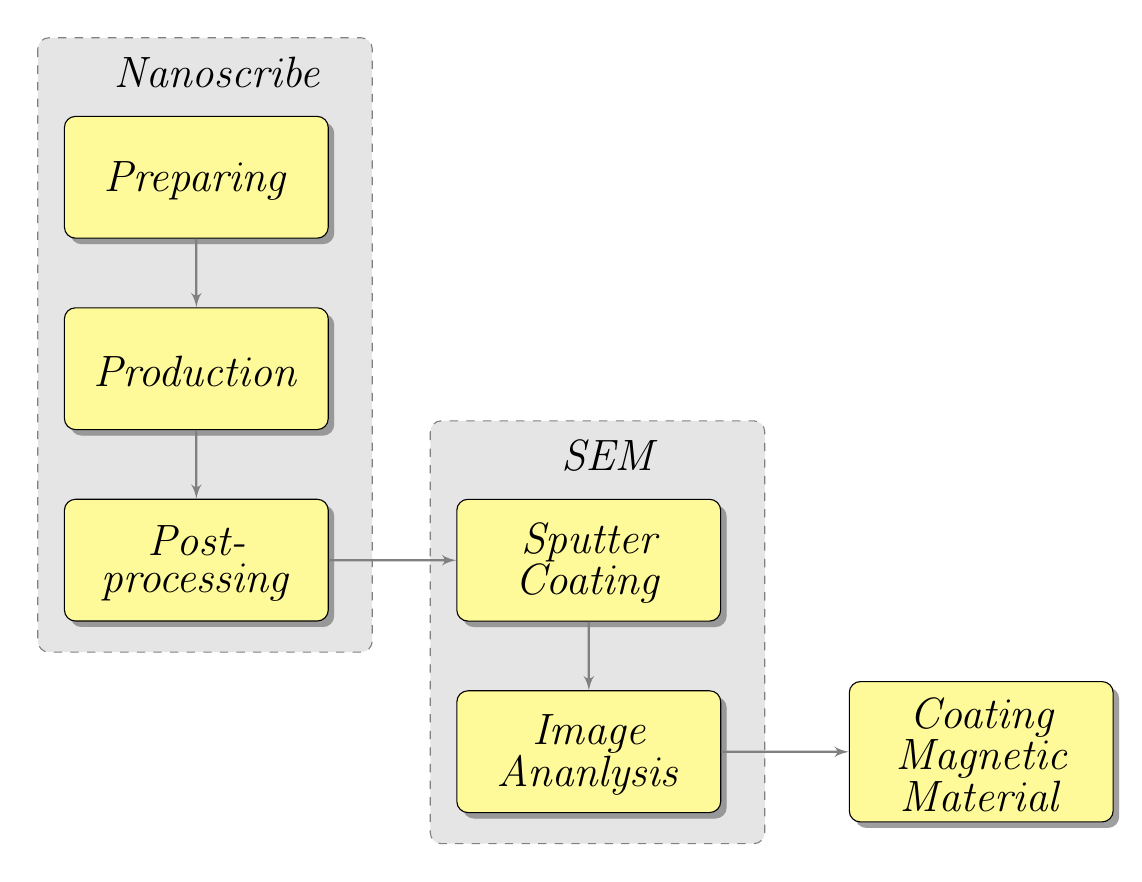
\begin{tikzpicture}[scale=1.10,transform shape]

  % Draw diagram elements
  \path \Step{1}{Preparing};
  \path (p1.south)+(0.0,-1.5) \Step{2}{Production};

  \path (p2.south)+(0.0,-1.5) \Step{3}{Post-processing};
  \path (p3.east)+(3.0,0.0) \Step{4}{Sputter Coating};
  \path (p4.south)+(0.0,-1.50) \Step{5}{Image Ananlysis};

 \path (p5.east)+(3.0,0.0) \Step{6}{Coating Magnetic Material};
  %\path (p4.east)+(5.0,0.0) \practica{7}{Calculate forward and inverse kinematic};
  %\path (p5.east)+(5.0,0.0) \practica{8}{Design feedback control mechanics};

  %\path (p5.south)+(3.5,-2.0) \practica{9}{Integrating e-AR and robot};
  %\path (p9.south)+(0.0,-1.5) \practica{10}{Laparoscopy Robot};


  % Draw arrows between elements
  \path [line] (p1.south) -- node [above] {} (p2);
  \path [line] (p2.south) -- node [above] {} (p3);
  \path [line] (p3.east) -- node [above] {} (p4);
  \path [line] (p4.south) -- node [above] {} (p5);

 \path [line] (p5.east) -- node [above] {} (p6);
%  \path [line] (p7.south) -- node [above] {} (p8);

  %\path [line] (p5.south) -- node [above] {} (p9);
  %\path [line] (p8.south) -- node [above] {} (p9);
 % \path [line] (p9.south) -- node [above] {} (p10);



  \background{p1}{p1}{p3}{p3}{Nanoscribe }
  \background{p4}{p4}{p5}{p5}{SEM}
  

 % \path [line] (p5.south) -- node [above] {} (bk3-n);
 % \path [line] (bk3-s) -- node [above] {} (p8);
 % \path [line] (bk3-s) -- node [above] {} (p9);
  %\path (bk1-e)+(+6.0,0) node (ur1)[ur] {};
 % \path (bk2-w)+(+6.0,0) node (ur2)[ur] {};
  %\path (bk3-w)+(+3.0,0) node (ur3)[ur] {};
% \transreceptor{bk1-e}{pre processing}{ur1};
 % \transreceptor{bk2-w}{Feature selection}{ur2};
  %\transreceptor{bk3-w}{classification}{ur3};


%%%%%%%%%%%%%% CHANGED%%%%%%%%%%%%%
\end{tikzpicture}									   %
\caption{Fabrication diagram. The nanoscribe technology is employed
for the fabrication process and it followed by analysing structure under SEM. 
The final stage (yellow block in third column) has not been tried in this project. }						   %
\label{Fabrication diagram}										   %
\end{figure}										   %	
												   %
%%%%%%%%%%%%%% CHANGED%%%%%%%%%%%%%




\paragraph{}

\begin{figure}
\centering
\begin{tikzpicture}[scale=1.15,transform shape]

  % Draw diagram elements
  \path \Step{1}{Propulsion Algorithm};
  \path (p1.south)+(0.0,-2.0) \Step{2}{Actuation Algorithm};

  \path (p2.south)+(0.0,-3.5) \Step{3}{Nanoscribe};
  \path (p3.south)+(0.0,-2.0) \Step{4}{SEM};
  \path (p6.west)+(-12.0,2.00) \Step{5}{Design};

 \path (p4.east)+(3.0,5.5) \Step{6}{Optimisation};
  %\path (p4.east)+(5.0,0.0) \practica{7}{Calculate forward and inverse kinematic};
  %\path (p5.east)+(5.0,0.0) \practica{8}{Design feedback control mechanics};

  %\path (p5.south)+(3.5,-2.0) \practica{9}{Integrating e-AR and robot};
  %\path (p9.south)+(0.0,-1.5) \practica{10}{Laparoscopy Robot};


  % Draw arrows between elements
  \path [line] (p1.south) -- node [above] {} (p2);
  \path [line] (p3.south) -- node [above] {} (p4);
 \path [line] (p5.north) -- node [above] {} (p1);
  \path [line] (p5.south) -- node [above] {} (p3);

 \path [line] (p4.east) -- node [above] {} (p6);
  \path [line] (p2.east) -- node [above] {} (p6);

  %\path [line] (p5.south) -- node [above] {} (p9);
  %\path [line] (p8.south) -- node [above] {} (p9);
 % \path [line] (p9.south) -- node [above] {} (p10);



  \background{p1}{p1}{p2}{p2}{Simulation }
  \background{p3}{p3}{p4}{p4}{Fabrication}

  

 % \path [line] (p5.south) -- node [above] {} (bk3-n);
 % \path [line] (bk3-s) -- node [above] {} (p8);
 % \path [line] (bk3-s) -- node [above] {} (p9);
  %\path (bk1-e)+(+6.0,0) node (ur1)[ur] {};
 % \path (bk2-w)+(+6.0,0) node (ur2)[ur] {};
  %\path (bk3-w)+(+3.0,0) node (ur3)[ur] {};
% \transreceptor{bk1-e}{pre processing}{ur1};
 % \transreceptor{bk2-w}{Feature selection}{ur2};
  %\transreceptor{bk3-w}{classification}{ur3};


%%%%%%%%%%%%%% CHANGED%%%%%%%%%%%%%
\end{tikzpicture}									   %
\caption{System Architecture.  }						   %
\label{System Architecture.}										   %
\end{figure}										   %	
												   %
%%%%%%%%%%%%%% CHANGED%%%%%%%%%%%%%


\end{document}